\section{Abhängigkeit der H--$\alpha $ Linie von der\\Spektralklasse}
Sterne sind anhand ihrer Spektrallinien in verschiedene Klassen unterteilt, Abb.\ (\ref{fig:spektralklasse}).
Mit Hilfe der H--$\alpha $ Linie lassen sich Aussagen über die Menge an Wasserstoff in einem Stern tätigen und damit auch über seine Eigenschaften und Entwicklung.
In diesem Versuch wird die Besetzungszahl der Elektronen im $n=2$ Niveau des Wasserstoffatoms berechnet und der Elektronendruck überprüft.

\begin{figure}[t]
  \centering
  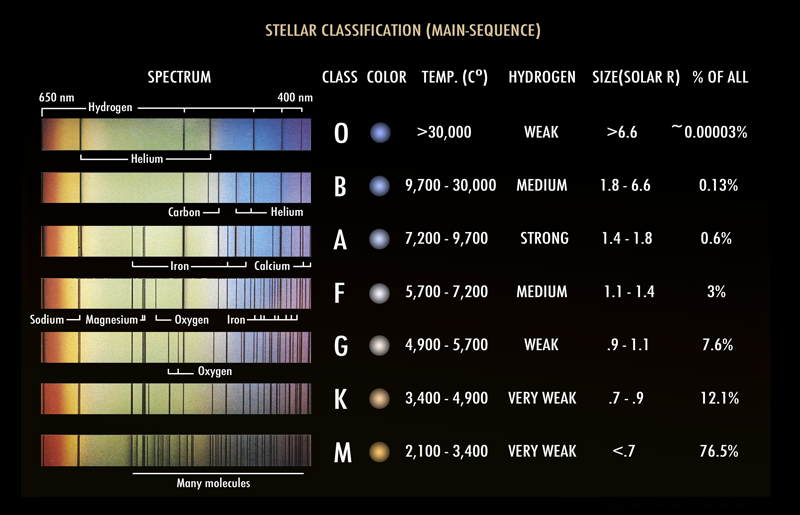
\includegraphics[width=.5\textwidth]{464_stellar_classification_chart.png}
  \caption{Spektralklassen der Sterne.\cite{wikipediaSpektralklasse}} \label{fig:spektralklasse}
\end{figure}
